\documentclass[runningheads]{llncs}
\usepackage{amsmath,amssymb,amsfonts}
\usepackage{graphicx}
\usepackage[hidelinks]{hyperref}
\usepackage{booktabs}
\usepackage{tikz}
\usetikzlibrary{arrows.meta, positioning}

\begin{document}

\title{The Externalization Horizon: An Information-Theoretic Boundary \\
for Internal States in Active Inference Systems}

\author{Alejandro Jimenez Rodriguez\inst{1} \and Mahault Albarracin\inst{1,2,3,4}}

\authorrunning{A. Jimenez Rodriguez, M. Albarracin}

\institute{
School of Computing and Digital Technologies, Sheffield Hallam University, Sheffield, United Kingdom \\
\email{a.jimenez@shu.ac.uk}
\and
LANCI -- Laboratoire d'Analyse Cognitive de l'Information, Universit\'{e} du Qu\'{e}bec \`{a} Montr\'{e}al, Canada \\
\email{mahault.albarracin@gmail.com}
\and
ISS -- Institut Sant\'{e} et Soci\'{e}t\'{e}, Universit\'{e} du Qu\'{e}bec \`{a} Montr\'{e}al, Canada
\and
IREF -- Institut de Recherches F\'{e}ministes, Universit\'{e} du Qu\'{e}bec \`{a} Montr\'{e}al, Canada
}

\maketitle

\begin{abstract}
Active inference agents maintain internal belief states that drive action selection through Expected Free Energy (EFE) minimization. A fundamental question for artificial general intelligence is: \emph{when can these internal states be inferred by external observers?} We introduce the \textbf{externalization horizon}: an information-theoretic boundary that separates \emph{readable} agents from \emph{dark} ones. Our key insight is that this boundary is \textbf{observer-dependent}: readability is not a property of the agent alone, but emerges from the \emph{similarity} between the observer's generative model and the agent's actual dynamics. The same agent can be transparent to one observer and opaque to another, depending on how well each observer's model matches the agent's internal parameters. We formalize this in the linear-Gaussian setting, where both the agent (Kalman-filter perception with EFE-optimal linear policy) and the observer (Kalman-filter-based Theory of Mind) perform principled active inference. We derive closed-form expressions for the externalization measure, show that policy gain mismatch dominates readability degradation through the observation model, and identify innovation consistency as a metric that detects model misspecification invisible to correlation. We validate these results with simulations and discuss implications for AGI interpretability, multi-agent coordination, and the boundary between communicable and private cognitive states.
\end{abstract}

\keywords{Active Inference \and Markov Blankets \and Information Theory \and Model Mismatch \and Theory of Mind \and Interpretability}

%% ============================================================
\section{Introduction}
\label{sec:intro}
%% ============================================================

A central challenge in artificial general intelligence concerns the relationship between an agent's internal cognitive states and its observable behavior. When can an external observer infer what an agent ``thinks''? When does an agent's internal model causally shape its environment? And under what conditions do internal states become effectively \emph{private}---causally disconnected from the observable world?

The Free Energy Principle (FEP) \cite{friston2006free,friston2010free} provides a principled framework for understanding agents as inference machines that maintain generative models of their environment. Under active inference \cite{parr2022active}, agents act to minimize Expected Free Energy (EFE), simultaneously reducing uncertainty about hidden states and fulfilling prior preferences \cite{parr2019generalized}. The Markov blanket \cite{pearl1988probabilistic,friston2013life} formalizes the boundary between agent and environment: internal states are conditionally independent of external states given the blanket (sensory and active states). This partition has been extended to hierarchical biological organization \cite{kirchhoff2018markov} and more recently to a physics of beliefs through Bayesian mechanics \cite{ramstead2023bayesian}.

However, the Markov blanket is a \emph{structural} property of a graphical model. It tells us that a boundary \emph{exists}, but not how much information actually flows through it. As Bruineberg et al.~\cite{bruineberg2022emperor} demonstrated in their influential critique, there is a persistent equivocation in the literature between ``Pearl blankets'' (epistemic tools for conditional independence) and ``Friston blankets'' (claimed physical boundaries of self-organizing systems). Raja et al.~\cite{raja2021free} further argued that the FEP presupposes rather than explains the agent-environment boundary. More technically, Biehl et al.~\cite{biehl2021technical} showed that various definitions of Markov blankets in FEP papers are not equivalent, and Aguilera et al.~\cite{aguilera2022particular} demonstrated that Markov blanket conditions hold only in a very narrow parameter space for linear stochastic systems, failing in the nonequilibrium regimes where living systems actually operate \cite{aguilera2023knitting}.

A door may exist between two rooms; the Markov blanket tells us the door is there, but not whether it is open, ajar, or sealed shut. Two agents may share identical graphical structure yet differ radically in how much their internal states influence---or are readable from---the environment, depending on noise levels, coupling strengths, and policy precision.

We propose the \textbf{externalization horizon}: a continuous, observer-dependent, information-theoretic boundary that determines when an agent's internal states are readable from the observable world. Our contributions are:

\begin{enumerate}
    \item We define \textbf{externalization} as the transfer entropy from beliefs to environment, deriving closed-form expressions in the linear-Gaussian case that decompose into coupling strength, belief variability, and noise.
    \item We show that the externalization horizon is \textbf{observer-dependent}: readability emerges from the \emph{similarity} between the observer's generative model and the agent's actual dynamics, not from a property of the agent alone. The same agent can be transparent to one observer and opaque to another.
    \item We identify \textbf{policy gain mismatch} as the dominant factor in readability degradation (through the observation model $H_B = \beta K_B$), and \textbf{innovation consistency} as a diagnostic that detects model misspecification invisible to correlation.
    \item We validate with simulations demonstrating observer-dependent horizons, dynamic opacity from parameter change, and feedback coupling as a special case of model mismatch.
\end{enumerate}

The externalization horizon provides a principled answer to questions that the Markov blanket framework alone cannot address: When is an AI system interpretable---and \emph{to whom}? When can agents model each other? What is the boundary between communicable and private cognitive states, and how does that boundary depend on the observer?

%% ============================================================
\section{Related Work}
\label{sec:related}
%% ============================================================

\paragraph{The Free Energy Principle and Markov Blankets.}
The FEP posits that self-organizing systems minimize variational free energy, maintaining themselves within expected states through perception and action \cite{friston2006free,friston2010free}. The Markov blanket formalism \cite{pearl1988probabilistic,friston2013life,kirchhoff2018markov} partitions system states into internal, external, sensory, and active states, providing a formal boundary for self-organization. Parr et al.~\cite{parr2020information} connected Markov blankets to information geometry and stochastic thermodynamics, showing that the blanket partition induces a dual information geometry. However, multiple critiques have demonstrated that the blanket's existence is a \emph{necessary but not sufficient} condition for cognitive agency \cite{bruineberg2022emperor,raja2021free,biehl2021technical,aguilera2022particular}. Most relevantly, Possati~\cite{possati2025density} recently proposed \emph{Markov blanket density}---a continuous scalar field $\rho \in [0,1]$ quantifying the \emph{degree} of conditional independence at each point---as a graded generalization of the binary blanket. Similarly, Sakthivadivel~\cite{sakthivadivel2022weak} introduced ``weak'' Markov blankets as an approximate, graded version. Our externalization horizon complements these efforts by quantifying information flow \emph{through} the blanket rather than the blanket's structural strength.

\paragraph{Empowerment and Intrinsic Motivation.}
Empowerment \cite{klyubin2005empowerment,salge2014empowerment} quantifies the channel capacity from an agent's actions to its future sensory states: $\mathfrak{E} = \max_{p(a)} I(a_t; s_{t+1})$. Kiefer~\cite{kiefer2025empowerment} recently proved that the generalized free energy used in active inference is equivalent to empowerment constrained by risk, unifying active inference, empowerment, and causal path entropy as variations on constrained maximum entropy inference. Our controllability measure $\mathcal{R}_a$ is closely related but richer: it measures information flow from \emph{beliefs} (not just actions) to the \emph{environment} (not just the agent's own sensors). Empowerment is a \emph{capacity} (optimized over action distributions); externalization is a \emph{rate} (under the actual policy). An agent may have high empowerment but low externalization if its policy does not exploit its action capacity.

\paragraph{Transfer Entropy and Causal Influence.}
Transfer entropy \cite{schreiber2000measuring} measures directed information flow between time series: $T_{X \to Y} = I(Y_{t+1}; X_t | Y_t)$. For Gaussian variables, transfer entropy is equivalent to Granger causality \cite{barnett2009granger}. Our externalization measure $I(\mu_t; e_{t+1} | e_t)$ is structurally identical to transfer entropy from beliefs to environment. Importantly, Ay and Polani~\cite{ay2008information} showed that information flow defined via interventional distributions (do-calculus) is not the same as statistical association---transfer entropy can vanish even when causal influence exists. Kolchinsky and Wolpert~\cite{kolchinsky2018semantic} defined \emph{semantic information} as the syntactic information causally necessary for a system to maintain its own existence, introducing a \emph{viability threshold} below which the agent cannot sustain itself---the closest existing formalism to our externalization horizon. Lizier et al.~\cite{lizier2008phase} demonstrated that transfer entropy peaks at phase transitions in random Boolean networks, showing that information transfer is maximized at the edge of chaos. We go beyond measuring information flow to identifying the critical threshold where this flow collapses, providing a named boundary concept.

\paragraph{Theory of Mind and Multi-Agent Inference.}
Theory of Mind (ToM) in artificial agents has been formalized through inverse planning \cite{baker2017rational}, meta-learning \cite{rabinowitz2018machine}, and active inference approaches to social cognition \cite{friston2015duet,veissiere2020thinking,vasil2020communication}. Friston and Frith~\cite{friston2015duet} showed that communication between agents can be modeled as coupled inference, where each agent inverts a generative model of the other's behavior. Maisto et al.~\cite{maisto2023interactive} operationalized this as ``interactive inference,'' where agents simultaneously minimize their own free energy and select actions that make their intentions \emph{legible} to others. Albarracin et al.~\cite{albarracin2024protentions} formalized shared anticipatory structures in multi-agent active inference using category theory, while Albarracin et al.~\cite{albarracin2026empathy} demonstrated that empathic perspective-taking through self-other model transformation induces robust cooperation in iterated games without explicit communication. Our framework provides a \emph{dual necessary condition} for all such social inference: an observer can model another agent's internal states only if (i)~the agent sufficiently externalizes (deposits information in the environment), AND (ii)~the observer's generative model of the agent is sufficiently accurate. Externalization is necessary but not sufficient---an observer with a misspecified model of the agent's dynamics will fail to read even heavily externalized states. This connects to the inverse reinforcement learning literature \cite{baker2017rational}, where inferring an agent's reward function requires a correct model of its planning algorithm.

\paragraph{Neurophenomenology and the Privacy of Experience.}
Generative neurophenomenology \cite{monnier2025generative} extends Varela's program \cite{varela1996neurophenomenology} to interpersonal settings, proposing that shared experience emerges through ``mutual incorporation'' in an ``interbeing space.'' Ramstead et al.~\cite{ramstead2022generative} formalized ``generative passages'' connecting phenomenological descriptions to neural mechanisms through the mathematical structure of generative models, while Sandved-Smith et al.~\cite{sandvedsmith2025deep} applied deep computational neurophenomenology to investigate the ``how'' of experience. Our framework formalizes the complementary question: when does mutual incorporation fail---when do two agents remain strangers despite interaction?

%% ============================================================
\section{Mathematical Framework}
\label{sec:math}
%% ============================================================

We begin with a minimal model that admits closed-form analysis, then generalize.

\subsection{A Simple Active Inference Agent}

Consider an agent with scalar internal state $x_t \in \mathbb{R}$, evolving as an AR(1) process with drift:
\begin{equation}
    x_{t+1} = \varphi \, x_t + v + \omega_t, \quad \omega_t \sim \mathcal{N}(0, \sigma_x^2)
    \label{eq:state_dynamics}
\end{equation}
where $\varphi \in [0,1)$ is the state persistence, $v$ is a drift term, and $\omega_t$ is process noise. The agent receives noisy observations:
\begin{equation}
    o_t = x_t + \xi_t, \quad \xi_t \sim \mathcal{N}(0, \sigma_o^2)
    \label{eq:observations}
\end{equation}

Under a Kalman filter---the optimal Bayesian estimator for this linear-Gaussian system, which can be derived as gradient descent on variational free energy in generalized coordinates \cite{friston2008variational,baltieri2020kalman}---the agent maintains a belief $\mu_t = \mathbb{E}[x_t \mid o_{1:t}]$ that evolves as:
\begin{equation}
    \mu_{t+1} = \varphi \mu_t + v + K_f(o_{t+1} - \varphi \mu_t - v)
    \label{eq:belief_update}
\end{equation}
where $K_f$ is the steady-state Kalman gain. The agent selects actions through a linear policy:
\begin{equation}
    a_t = K \mu_t
    \label{eq:policy}
\end{equation}
where $K$ is the policy gain, mapping beliefs to actions. This linear policy structure emerges from EFE minimization in the linear-Gaussian case, which reduces to KL control---the risk term dominates since the epistemic (ambiguity) term becomes constant with respect to additive control inputs \cite{koudahl2021efe,baltieri2020kalman}. The resulting optimal policy is a linear feedback law identical in form to LQR, where the precision of the preferred distribution encodes the cost on state deviations.

\subsection{Agent-Environment Coupling}

The crucial step is to model an \emph{environment} that is influenced by the agent's actions. Let the environment state $e_t \in \mathbb{R}$ evolve as:
\begin{equation}
    e_{t+1} = \rho \, e_t + \beta \, a_t + \varepsilon_t, \quad \varepsilon_t \sim \mathcal{N}(0, \sigma_e^2)
    \label{eq:environment}
\end{equation}
where $\rho \in [0,1)$ is the autoregressive persistence of the environment, $\beta$ is the coupling strength from agent actions to environment, and $\varepsilon_t$ is environment noise. Substituting the policy (\ref{eq:policy}):
\begin{equation}
    e_{t+1} = \rho \, e_t + \underbrace{\beta K}_{\text{effective coupling}} \mu_t + \varepsilon_t
    \label{eq:env_with_beliefs}
\end{equation}

This is the key equation: the agent's \emph{internal belief} $\mu_t$ now appears directly in the environment dynamics. The product $\beta K$ determines the effective coupling---how strongly the agent's model of the world actually shapes the world.

\subsection{The Externalization Measure}

We define the \textbf{externalization} of the agent's internal state as the transfer entropy from beliefs to environment:
\begin{equation}
    \mathcal{E}(\mu \to e) \triangleq I(\mu_t; \, e_{t+1} \mid e_t)
    \label{eq:externalization}
\end{equation}

This measures how much additional information the agent's belief provides about the next environment state, beyond what the current environment state already provides. In the linear-Gaussian case, we can compute this in closed form.

\begin{proposition}[Closed-Form Externalization]
\label{prop:closed_form}
For the linear-Gaussian system defined by (\ref{eq:state_dynamics})--(\ref{eq:environment}), the externalization is:
\begin{equation}
    \mathcal{E}(\mu \to e) = \frac{1}{2} \log \left( 1 + \frac{\beta^2 K^2 \, \mathrm{Var}(\mu_t \mid e_t)}{\sigma_e^2} \right)
    \label{eq:externalization_closed}
\end{equation}
\end{proposition}

\begin{proof}
Conditioned on $e_t$, the next environment state is $e_{t+1} = \rho \, e_t + \beta K \mu_t + \varepsilon_t$. Since $\rho \, e_t$ is deterministic given $e_t$, the residual innovation is $\tilde{e}_{t+1} = \beta K \mu_t + \varepsilon_t$. The conditional mutual information between $\mu_t$ and $\tilde{e}_{t+1}$ (given $e_t$) follows the standard Gaussian channel formula \cite{cover2006elements}:
\[
I(\mu_t; \tilde{e}_{t+1} \mid e_t) = \frac{1}{2} \log \left( 1 + \frac{(\beta K)^2 \, \mathrm{Var}(\mu_t \mid e_t)}{\sigma_e^2} \right)
\]
where $\mathrm{Var}(\mu_t \mid e_t)$ is the conditional variance of the belief given the environment state. Since the transformation from $(\mu_t, \varepsilon_t)$ to $(e_{t+1})$ is affine given $e_t$, we have $I(\mu_t; e_{t+1} \mid e_t) = I(\mu_t; \tilde{e}_{t+1} \mid e_t)$.
\end{proof}

The externalization depends on three factors:
\begin{itemize}
    \item \textbf{Effective coupling} $\beta K$: the product of environment susceptibility and policy gain.
    \item \textbf{Belief variability} $\mathrm{Var}(\mu_t \mid e_t)$: how much the belief varies independently of the environment.
    \item \textbf{Environment noise} $\sigma_e^2$: how much the environment is driven by its own stochasticity.
\end{itemize}

\subsection{Observer-Dependent Readability}
\label{sec:readability}

The externalization measure $\mathcal{E}(\mu \to e)$ quantifies how much information agent $A$ \emph{deposits} into the environment. But a fundamental question remains: \emph{who can read it?} We now show that readability is not a property of the agent alone, but depends on the \emph{similarity} between the observer's generative model and the agent's actual dynamics.

Consider an observer $B$ who observes the environment with noise:
\begin{equation}
    o^B_t = e_t + \eta_t, \quad \eta_t \sim \mathcal{N}(0, \sigma_B^2)
    \label{eq:obs_B}
\end{equation}
Agent $B$ seeks to infer $A$'s beliefs $\mu^A_t$ by maintaining a generative model of $A$'s dynamics. Under active inference, this constitutes \emph{sophisticated inference}~\cite{friston2015duet}: $B$ minimizes variational free energy over a model of $A$'s internal states. In the linear-Gaussian case, $B$'s generative model takes the form:
\begin{align}
    s_{t+1} &= \varphi_B \, s_t + v_B + w_t, \quad w_t \sim \mathcal{N}(0, Q_B) \label{eq:tom_B_transition} \\
    z_t &= H_B \, s_t + \varepsilon_t, \quad \varepsilon_t \sim \mathcal{N}(0, R_B) \label{eq:tom_B_observation}
\end{align}
where $s_t$ is $B$'s estimate of $A$'s hidden belief state, $z_t = o^B_{t+1} - \rho \, o^B_t$ is the innovation $B$ extracts from consecutive environment observations, $\varphi_B$ is $B$'s assumed belief persistence for $A$, $v_B$ is $B$'s assumed drift, and:
\begin{equation}
    H_B = \beta K_B, \quad R_B = \sigma_e^2 + \sigma_B^2(1 + \rho^2)
    \label{eq:H_B}
\end{equation}
with $K_B$ being $B$'s assumed policy gain for $A$. The process noise $Q_B$ is derived from $B$'s assumed Kalman gain and prediction variance for $A$'s filter.

The crucial point is that $B$'s model parameters $\boldsymbol{\theta}_B = (\varphi_B, v_B, K_B)$ may differ from $A$'s actual parameters $\boldsymbol{\theta}_A = (\varphi, v, K)$. The \textbf{model mismatch vector} is:
\begin{equation}
    \boldsymbol{\delta} = \boldsymbol{\theta}_B - \boldsymbol{\theta}_A = (\delta_\varphi, \delta_v, \delta_K)
    \label{eq:mismatch}
\end{equation}

VFE minimization over $q(s_t) = \mathcal{N}(m^B_t, P^B_t)$ yields a Kalman filter---the exact solution in the LG case. When $\boldsymbol{\delta} = \mathbf{0}$ (matched model), $B$'s inference is optimal: $m^B_t$ tracks $\mu^A_t$ with accuracy limited only by observation noise. When $\boldsymbol{\delta} \neq \mathbf{0}$ (misspecified model), $B$'s inference degrades systematically.

\begin{proposition}[Observer-Dependent Readability]
\label{prop:readability}
The readability of agent $A$ by observer $B$, measured as $R^2(\mu^A, m^B)$, satisfies:
\begin{enumerate}
    \item $R^2$ peaks at $\boldsymbol{\delta} = \mathbf{0}$ (matched model) and decays with $|\boldsymbol{\delta}|$.
    \item Policy gain mismatch $\delta_K$ dominates readability degradation, because $K_B$ enters $B$'s \emph{observation model} $H_B = \beta K_B$, directly scaling the signal $B$ expects to see.
    \item Persistence mismatch $\delta_\varphi$ affects only $B$'s \emph{transition model}, producing subtler degradation detectable through the \textbf{innovation consistency ratio} $\mathrm{ICR} = \mathrm{Var}(\text{innov})/S$, which departs from $1$ under misspecification even when $R^2$ remains high.
\end{enumerate}
\end{proposition}

The \textbf{externalization horizon} is now defined as a boundary in model space:
\begin{equation}
    \mathcal{H}(A) = \left\{ \boldsymbol{\theta}_B : R^2\!\left(\mu^A, m^B(\boldsymbol{\theta}_B)\right) = r_s \right\}
    \label{eq:horizon_model_space}
\end{equation}
where $r_s$ is the readability threshold and $R^2$ denotes a readability metric. In practice, the coefficient of determination $\mathrm{CoD} = 1 - \mathrm{MSE}/\mathrm{Var}(\mu^A)$ is preferable to the squared correlation $\mathrm{corr}^2$, because the latter is scale-invariant and fails to penalize the systematic bias and scale errors that arise when $K_B \neq K_A$ (Section~\ref{sec:simulations}). This is a closed surface around the matched point $\boldsymbol{\theta}_A$ in parameter space. The same agent $A$ is readable to observers inside $\mathcal{H}(A)$ and dark to observers outside it. The horizon's shape reveals which model parameters matter most: it is narrow in the $K$-direction (high sensitivity) and wider in the $\varphi$-direction (lower sensitivity).

\subsection{Feedback as Model Mismatch}
\label{sec:feedback_mismatch}

In realistic settings, the environment feeds back into the agent's state:
\begin{equation}
    x_{t+1} = \varphi \, x_t + \alpha \, e_t + v + \omega_t
    \label{eq:state_feedback}
\end{equation}
where $\alpha$ quantifies the feedback coupling. An \textbf{$\alpha$-aware agent} incorporates an environment estimate $\hat{e}_t$ into its prediction, modifying its effective transition dynamics. An observer $B$ who assumes $\alpha = 0$ has a \emph{structurally misspecified model}: $B$'s assumed transition $\varphi_B s_t + v_B$ omits the feedback term that shapes $A$'s actual belief trajectory.

This reframes the naive/aware distinction as a special case of model mismatch. Different metrics have different sensitivity to this type of misspecification:
\begin{itemize}
    \item \textbf{$R^2$ correlation} is insensitive to transition model errors: both the naive observer ($\alpha_B = 0$) and a matched observer ($\alpha_B = \alpha$) achieve similar $R^2$, because the Kalman filter's observation update compensates for one-step prediction errors.
    \item \textbf{Innovation consistency ratio} $\mathrm{ICR} = \mathrm{Var}(\text{innov})/S$ clearly separates the two: the naive observer's innovations are systematically larger than predicted ($\mathrm{ICR} > 1$), while the matched observer maintains $\mathrm{ICR} \approx 1$.
\end{itemize}

This suggests that the externalization horizon has \textbf{two layers}: a \emph{correlation horizon} where $R^2$ drops below threshold (requiring large mismatch, typically in $K$), and a \emph{calibration horizon} where innovation consistency degrades (detectable at smaller mismatch, particularly in $\varphi$ or $\alpha$). An observer may be ``above'' the correlation horizon but ``below'' the calibration horizon---able to track the agent's beliefs in a correlational sense but unable to detect that its own model is wrong.

%% ============================================================
\section{The Externalization Horizon}
\label{sec:horizon}
%% ============================================================

\subsection{Controllability and Observability}

We now generalize beyond instantaneous externalization to define two complementary infinite-horizon measures, following the intuition from control theory \cite{baltieri2020bayesian}.

\begin{definition}[Controllability]
The \textbf{controllability radius} of an internal state $s_t$ is:
\begin{equation}
    \mathcal{R}_a(s_t) = I(s_t; \, Y_{t+1:\infty})
    \label{eq:controllability}
\end{equation}
where $Y_{t+1:\infty}$ denotes the future trajectory of the environment. This measures how much the current internal state causally influences all future environment states.
\end{definition}

\begin{definition}[Observability]
The \textbf{observability radius} of an internal state $s_t$ is:
\begin{equation}
    \mathcal{R}_o(s_t) = I(s_t; \, O^B_{t+1:\infty})
    \label{eq:observability}
\end{equation}
where $O^B_{t+1:\infty}$ denotes the future observations available to an external observer $B$. This measures how much an observer could, in principle, infer about the agent's internal state.
\end{definition}

In general, observability is bounded by controllability:
\begin{equation}
    \mathcal{R}_o(s_t) \leq \mathcal{R}_a(s_t)
    \label{eq:obs_leq_ctrl}
\end{equation}
since an observer can only infer internal states through their causal traces in the environment (a consequence of the data processing inequality \cite{cover2006elements}). Equality holds when the observer has noiseless access to all environment states influenced by the agent.

\subsection{The Critical Threshold}

\begin{definition}[Externalization Horizon]
An internal state $s_t$ is \textbf{beyond the externalization horizon} if its controllability falls below a critical threshold $r_s$:
\begin{equation}
    \mathcal{R}_a(s_t) < r_s
    \label{eq:horizon_condition}
\end{equation}
where $r_s$ is the minimum information rate required for the state to have a detectable causal footprint in the environment.
\end{definition}

For the linear-Gaussian model, we can compute $\mathcal{R}_a$ in closed form. Since the environment is an AR(1) process driven by the agent's beliefs, the total future influence decays geometrically:

\begin{proposition}[Controllability Radius]
\label{prop:controllability}
For the linear-Gaussian system with $|\rho| < 1$:
\begin{equation}
    \mathcal{R}_a(s_t) = \frac{1}{2} \sum_{k=0}^{\infty} \log \left(1 + \frac{\rho^{2k} \beta^2 K^2 \, \mathrm{Var}(\mu_{t+k} \mid e_{t+k})}{\sigma_e^2} \right)
    \label{eq:controllability_series}
\end{equation}
Under stationarity (constant $\mathrm{Var}(\mu \mid e) = \sigma_\mu^2$), this simplifies to:
\begin{equation}
    \mathcal{R}_a \approx \frac{1}{2(1-\rho^2)} \log \left( 1 + \frac{\beta^2 K^2 \sigma_\mu^2}{\sigma_e^2} \right)
    \label{eq:controllability_approx}
\end{equation}
\end{proposition}

The horizon condition $\mathcal{R}_a < r_s$ then yields:

\begin{corollary}[Horizon Condition]
Internal states fall beyond the externalization horizon when:
\begin{equation}
    \beta K < \frac{\sigma_e}{\sigma_\mu} \sqrt{e^{2 r_s (1-\rho^2)} - 1}
    \label{eq:horizon_bk}
\end{equation}
\end{corollary}

This reveals the \textbf{trivial horizons}:
\begin{itemize}
    \item $\beta K = 0$: The agent has no causal impact on the environment (zero coupling or zero policy gain). All internal states are dark.
    \item $\sigma_e^2 \to \infty$: The environment is so noisy that any agent influence is drowned out.
    \item $\sigma_\mu^2 \to 0$: The agent's beliefs carry no private information beyond what the environment already determines.
\end{itemize}

\subsection{Phase Transition}

The externalization exhibits a sharp transition as a function of the effective signal-to-noise ratio $\text{SNR} = \beta^2 K^2 \sigma_\mu^2 / \sigma_e^2$:

\begin{equation}
    \mathcal{E} = \frac{1}{2} \log(1 + \text{SNR}) \approx
    \begin{cases}
        \frac{\text{SNR}}{2} & \text{if } \text{SNR} \ll 1 \quad \text{(dark regime)} \\
        \frac{1}{2} \log(\text{SNR}) & \text{if } \text{SNR} \gg 1 \quad \text{(transparent regime)}
    \end{cases}
    \label{eq:phase_transition}
\end{equation}

In the dark regime, externalization grows linearly with coupling---small changes barely register. In the transparent regime, externalization grows logarithmically---the agent's internal states are already substantially readable, and further coupling yields diminishing returns. The transition between regimes occurs at $\text{SNR} \approx 1$, defining a natural critical point.

%% ============================================================
\section{Multi-Agent Extension}
\label{sec:multi_agent}
%% ============================================================

We now extend the framework to consider an observer agent $B$ attempting to infer the internal states of agent $A$.

\subsection{Two Observation Regimes}

Following the standard active inference perception-action loop for agent $A$:
\begin{equation}
    \mu_t^A \to a_t^A \to o_{t+1}^A \to \mu_{t+1}^A
    \label{eq:agent_loop}
\end{equation}

We distinguish two scenarios for observer $B$:

\paragraph{Scenario (i): Environment Screen.}
Observer $B$ only accesses the environment state, not agent $A$'s actions directly:
\begin{equation}
    \mu_t^A \to a_t^A \to \underbrace{e_{t+1}}_{\text{environment}} \to o_{t+1}^B
    \label{eq:screen}
\end{equation}
The environment acts as a ``screen'' that mediates all information. By the data processing inequality, the observer's inference is strictly limited:
\begin{equation}
    I(\mu_t^A; \, o_{t+1}^B) \leq I(\mu_t^A; \, e_{t+1}) = \mathcal{E}(\mu^A \to e)
    \label{eq:screen_bound}
\end{equation}
If the observer's own sensory noise is $\sigma_B^2$, the observable externalization is:
\begin{equation}
    \mathcal{E}_{\text{screen}} = \frac{1}{2} \log \left( 1 + \frac{\beta^2 K^2 \sigma_\mu^2}{\sigma_e^2 + \sigma_B^2} \right)
    \label{eq:screen_externalization}
\end{equation}

\paragraph{Scenario (ii): Direct Behavioral Access.}
Observer $B$ can directly observe agent $A$'s actions:
\begin{equation}
    \mu_t^A \to a_t^A \to o_{t+1}^B \to \hat{\mu}_{t+1}^A
    \label{eq:direct}
\end{equation}
where $\hat{\mu}^A$ denotes $B$'s estimate of $A$'s beliefs. Since $a_t^A = K \mu_t^A + \eta_t$ (with action noise $\eta_t \sim \mathcal{N}(0, \sigma_\eta^2)$), the observable externalization is:
\begin{equation}
    \mathcal{E}_{\text{direct}} = \frac{1}{2} \log \left( 1 + \frac{K^2 \sigma_\mu^2}{\sigma_\eta^2} \right)
    \label{eq:direct_externalization}
\end{equation}
This depends on $K$ (policy gain) but not $\beta$ (environment coupling)---the observer bypasses the environment channel. This scenario connects to the legibility literature in human-robot interaction \cite{dragan2013legibility,maisto2023interactive}: legible behavior corresponds to high $\mathcal{E}_{\text{direct}}$, achieved through large policy gain $K$ and low action noise $\sigma_\eta$.

\subsection{Conditions for Theory of Mind}

Theory of Mind---the ability of observer $B$ to maintain a model of agent $A$'s beliefs \cite{friston2015duet}---requires \emph{two} conditions to be jointly satisfied:

\begin{proposition}[Dual ToM Condition]
\label{prop:dual_tom}
An observer $B$ can maintain a non-trivial model of agent $A$'s internal states only if:
\begin{enumerate}
    \item \textbf{Sufficient externalization}: $\mathcal{E}_{\text{obs}} > r_s^B$, where $\mathcal{E}_{\text{obs}}$ is the externalization available to $B$ (via screen or direct access, eqs.~\ref{eq:screen_externalization}--\ref{eq:direct_externalization}) and $r_s^B$ is $B$'s inference threshold.
    \item \textbf{Sufficient model match}: $\boldsymbol{\theta}_B \in \mathcal{H}(A)$, i.e., $B$'s assumed parameters lie within the horizon surface (eq.~\ref{eq:horizon_model_space}) defined in Section~\ref{sec:readability}.
\end{enumerate}
\end{proposition}

The first condition---\emph{you cannot model what you cannot observe}---is necessary but not sufficient. An agent whose externalization exceeds threshold deposits readable information in the environment, but an observer with a misspecified model of the agent's dynamics will fail to extract it. The second condition formalizes this: $B$'s generative model (eqs.~\ref{eq:tom_B_transition}--\ref{eq:tom_B_observation}) must be sufficiently similar to $A$'s actual dynamics for VFE minimization to produce accurate inference.

This dual condition connects to Veissi\`{e}re et al.'s observation that we think \emph{through} other minds \cite{veissiere2020thinking}: such thinking requires not only that the other mind be externalized, but that we have an adequate model of \emph{how} it externalizes. The observation gain $H_B = \beta K_B$ in $B$'s generative model (eq.~\ref{eq:H_B}) determines how $B$ maps innovations to belief estimates; when $K_B \neq K$, $B$'s VFE-minimizing Kalman filter converges to a systematically biased estimate of $A$'s beliefs, even though the filter itself is performing exact inference under its (wrong) model.

\subsection{Observer-Dependent Horizons}
\label{sec:observer_horizons}

The relational nature of readability means that each observer has a \emph{different} horizon for the same agent. Consider agent $A$ with fixed parameters $\boldsymbol{\theta}_A$ and two observers $B_1$, $B_2$ with parameters $\boldsymbol{\theta}_{B_1}$, $\boldsymbol{\theta}_{B_2}$:
\begin{equation}
    R^2(A, B_1) \neq R^2(A, B_2) \quad \text{even though } A \text{ is unchanged}
    \label{eq:observer_dependent}
\end{equation}

A well-calibrated observer ($\boldsymbol{\theta}_{B_1} \approx \boldsymbol{\theta}_A$) achieves high $R^2$ at lower coupling $\beta K$, while a miscalibrated observer ($|\boldsymbol{\theta}_{B_2} - \boldsymbol{\theta}_A|$ large) requires much stronger externalization to cross the readability threshold. This means the \emph{effective} externalization horizon depends on the observer: agent $A$ can be simultaneously transparent to $B_1$ and dark to $B_2$.

\subsection{Shared Externalization and the Interbeing Space}

When two agents mutually externalize---each influencing the environment that the other observes---a \emph{shared externalization space} emerges. Define the \textbf{mutual readability}:
\begin{equation}
    \mathcal{M}(A, B) = \min\left(R^2(A, B), \, R^2(B, A)\right)
    \label{eq:mutual_readability}
\end{equation}
where $R^2(A, B)$ is $B$'s inference quality about $A$'s beliefs. Note that mutual readability depends on \emph{both} agents' externalization AND \emph{both} agents' models of each other---it is doubly relational. This connects to the ``interbeing space'' of generative neurophenomenology \cite{monnier2025generative}: meaningful interpersonal experience requires that both agents' internal states be sufficiently externalized \emph{and} that each has an adequate model of the other.

When $\mathcal{M}(A, B) < r_s$, the agents interact mechanically (through environment coupling) but cannot engage in participatory sense-making---they remain strangers despite physical proximity.

%% ============================================================
\section{Distinguishing from the Markov Blanket}
\label{sec:vs_mb}
%% ============================================================

We now make precise the relationship between the externalization horizon and the Markov blanket. The key distinctions are summarized in Table~\ref{tab:comparison}.

\begin{table}[htbp]
\centering
\caption{Comparison of the Markov blanket and the externalization horizon.}
\label{tab:comparison}
\begin{tabular}{@{}lll@{}}
\toprule
\textbf{Property} & \textbf{Markov Blanket} & \textbf{Externalization Horizon} \\
\midrule
Nature & Structural (graph) & Quantitative (information) \\
Type & Conditional independence & Information flow rate \\
Scale & Binary (exists / doesn't) & Continuous ($\mathcal{E} \in [0, \infty)$) \\
Parameter dep. & No & Yes ($\beta, K, \sigma_e, \sigma_\mu$) \\
Phase transitions & No & Yes (SNR $\approx 1$) \\
Ctrl vs.\ obs & Conflated & Separated ($\mathcal{R}_a \neq \mathcal{R}_o$) \\
Observer dep. & No & Yes ($\boldsymbol{\theta}_B$) \\
\bottomrule
\end{tabular}
\end{table}

The Markov blanket is a necessary condition for externalization: if no blanket exists (no boundary at all), externalization is undefined. But the blanket's existence is \emph{not sufficient} to guarantee that internal states have any causal footprint. A robot with sensors and actuators has a Markov blanket, but if its policy gain $K \to 0$ (it ignores its beliefs) or the environment noise $\sigma_e^2 \to \infty$ (the world drowns out its actions), its internal states are effectively dark.

Our work is complementary to Possati's~\cite{possati2025density} Markov blanket density, which quantifies the \emph{structural strength} of the blanket partition (how close to perfect conditional independence), while our externalization horizon quantifies the \emph{functional consequence} of whatever blanket exists (how much information actually flows through it). An agent may have a strong blanket (high $\rho$ in Possati's framework) and yet low externalization (if the through-blanket coupling $\beta K$ is weak), or vice versa.

%% ============================================================
\section{Simulations}
\label{sec:simulations}
%% ============================================================

We validate the analytical results through simulations of active inference agents with Kalman-filter-based Theory of Mind.\footnote{Code available at \url{https://github.com/[anonymized]/externalization-horizon}.} Agent~$A$ performs VFE minimization (Kalman filtering) for perception and uses the EFE-optimal linear policy $a_t = K \mu_t$ \cite{baltieri2020kalman}. Observer~$B$ maintains a generative model of $A$'s belief dynamics (eqs.~\ref{eq:tom_B_transition}--\ref{eq:tom_B_observation}) and minimizes VFE via a Kalman filter---sophisticated inference over $A$'s hidden states. Transfer entropy is estimated via the Gaussian regression method: $\hat{\mathcal{E}} = \frac{1}{2}\log\bigl(\text{Var}(e_{t+1} \mid e_t) / \text{Var}(e_{t+1} \mid e_t, \mu_t)\bigr)$. Default parameters: $\varphi = 0.7$, $v = 0.3$, $K = 1$, $\rho = 0.5$, $\sigma_x = \sigma_o = \sigma_e = 1$.

\subsection{Externalization of an EFE-Optimal Agent}

Figure~\ref{fig:efe_ext} establishes the fundamental result: how much information an EFE-optimal active inference agent deposits into the environment. Panel~(a) shows transfer entropy $\mathcal{E}$ as a function of coupling strength $\beta K$, with analytical predictions from Proposition~\ref{prop:closed_form} closely matched by empirical estimates ($T = 20{,}000$). Panel~(b) reveals the \emph{phase transition} in signal-to-noise ratio (SNR) space. The externalization follows $\mathcal{E} = \frac{1}{2}\ln(1 + \text{SNR})$, which interpolates between two regimes: a \emph{dark regime} (SNR $\ll 1$) where externalization grows linearly with coupling and internal states are effectively private, and a \emph{transparent regime} (SNR $\gg 1$) where externalization grows logarithmically and beliefs are readable. The critical point at $\text{SNR} = 1$ defines a natural phase boundary---the externalization horizon in its simplest form.

\begin{figure}[htbp]
    \centering
    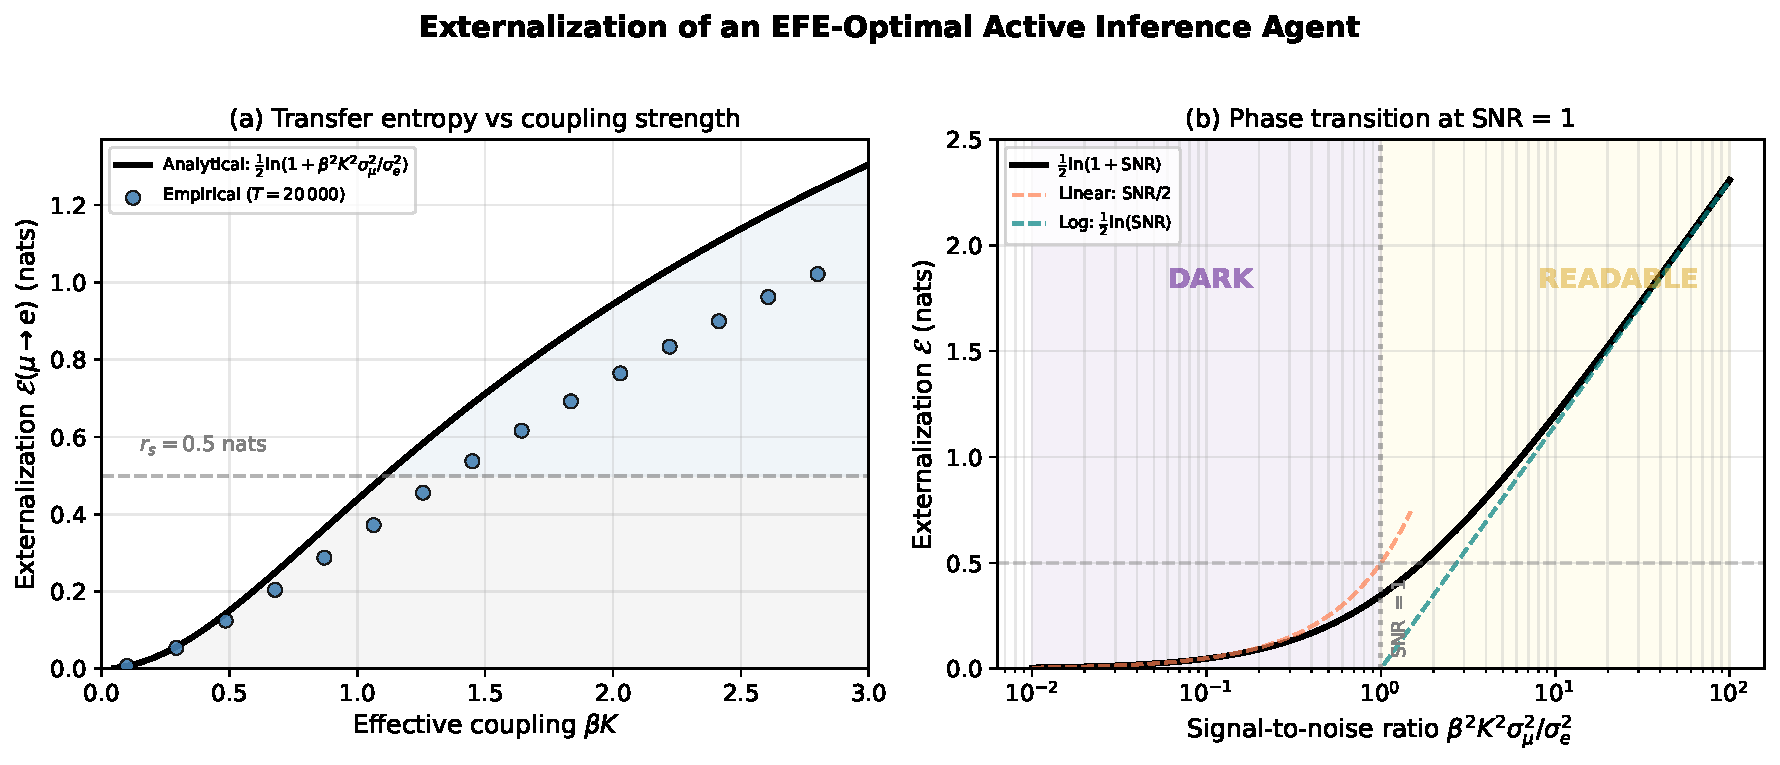
\includegraphics[width=\textwidth]{figures/fig1_efe_externalization.pdf}
    \caption{Externalization of an EFE-optimal active inference agent. (a)~Transfer entropy $\mathcal{E}(\mu \to e)$ vs effective coupling $\beta K$: analytical predictions (solid) match empirical estimates (dots, $T = 20{,}000$). (b)~Phase transition at $\text{SNR} = 1$: dark regime (left, linear growth) vs transparent regime (right, logarithmic growth). The agent performs VFE minimization for perception and EFE-optimal action $a_t = K\mu_t$.}
    \label{fig:efe_ext}
\end{figure}

\subsection{The Externalization Horizon in Model Space}

Figure~\ref{fig:horizon} is the centerpiece result: the externalization horizon visualized as a boundary in model-mismatch space. Each panel shows the coefficient of determination $\mathrm{CoD}(\varphi_B, K_B) = 1 - \mathrm{MSE}/\mathrm{Var}(\mu^A)$ across a $35 \times 35$ grid ($T = 3{,}000$ per simulation), with observer $B$ performing VFE-based sophisticated inference over agent $A$'s belief dynamics. Unlike $R^2 = \mathrm{corr}^2$ (which is scale-invariant and fails to penalize gain mismatch), the CoD properly penalizes bias and scale errors---exactly the pathology that arises when $K_B \neq K_A$. The white contour at $\mathrm{CoD} = r_s = 0.5$ defines the horizon surface $\mathcal{H}(A)$ (eq.~\ref{eq:horizon_model_space}). Panel~(a): at moderate coupling ($\beta = 1.5$, $\sigma_B = 0.5$), a majority of model space falls below the readability threshold---observers whose generative model of the agent diverges from reality cannot extract belief information despite performing exact VFE minimization under their (wrong) model. Panel~(b): at strong coupling ($\beta = 3.0$), the dark region shrinks dramatically. The horizon \emph{contracts} as coupling increases: stronger externalization compensates for model mismatch, making the agent readable to a wider range of observers. The ``inferno'' colormap (black $\to$ red $\to$ yellow) deliberately evokes the visual metaphor: the horizon is a boundary between darkness and light in model space.

\begin{figure}[htbp]
    \centering
    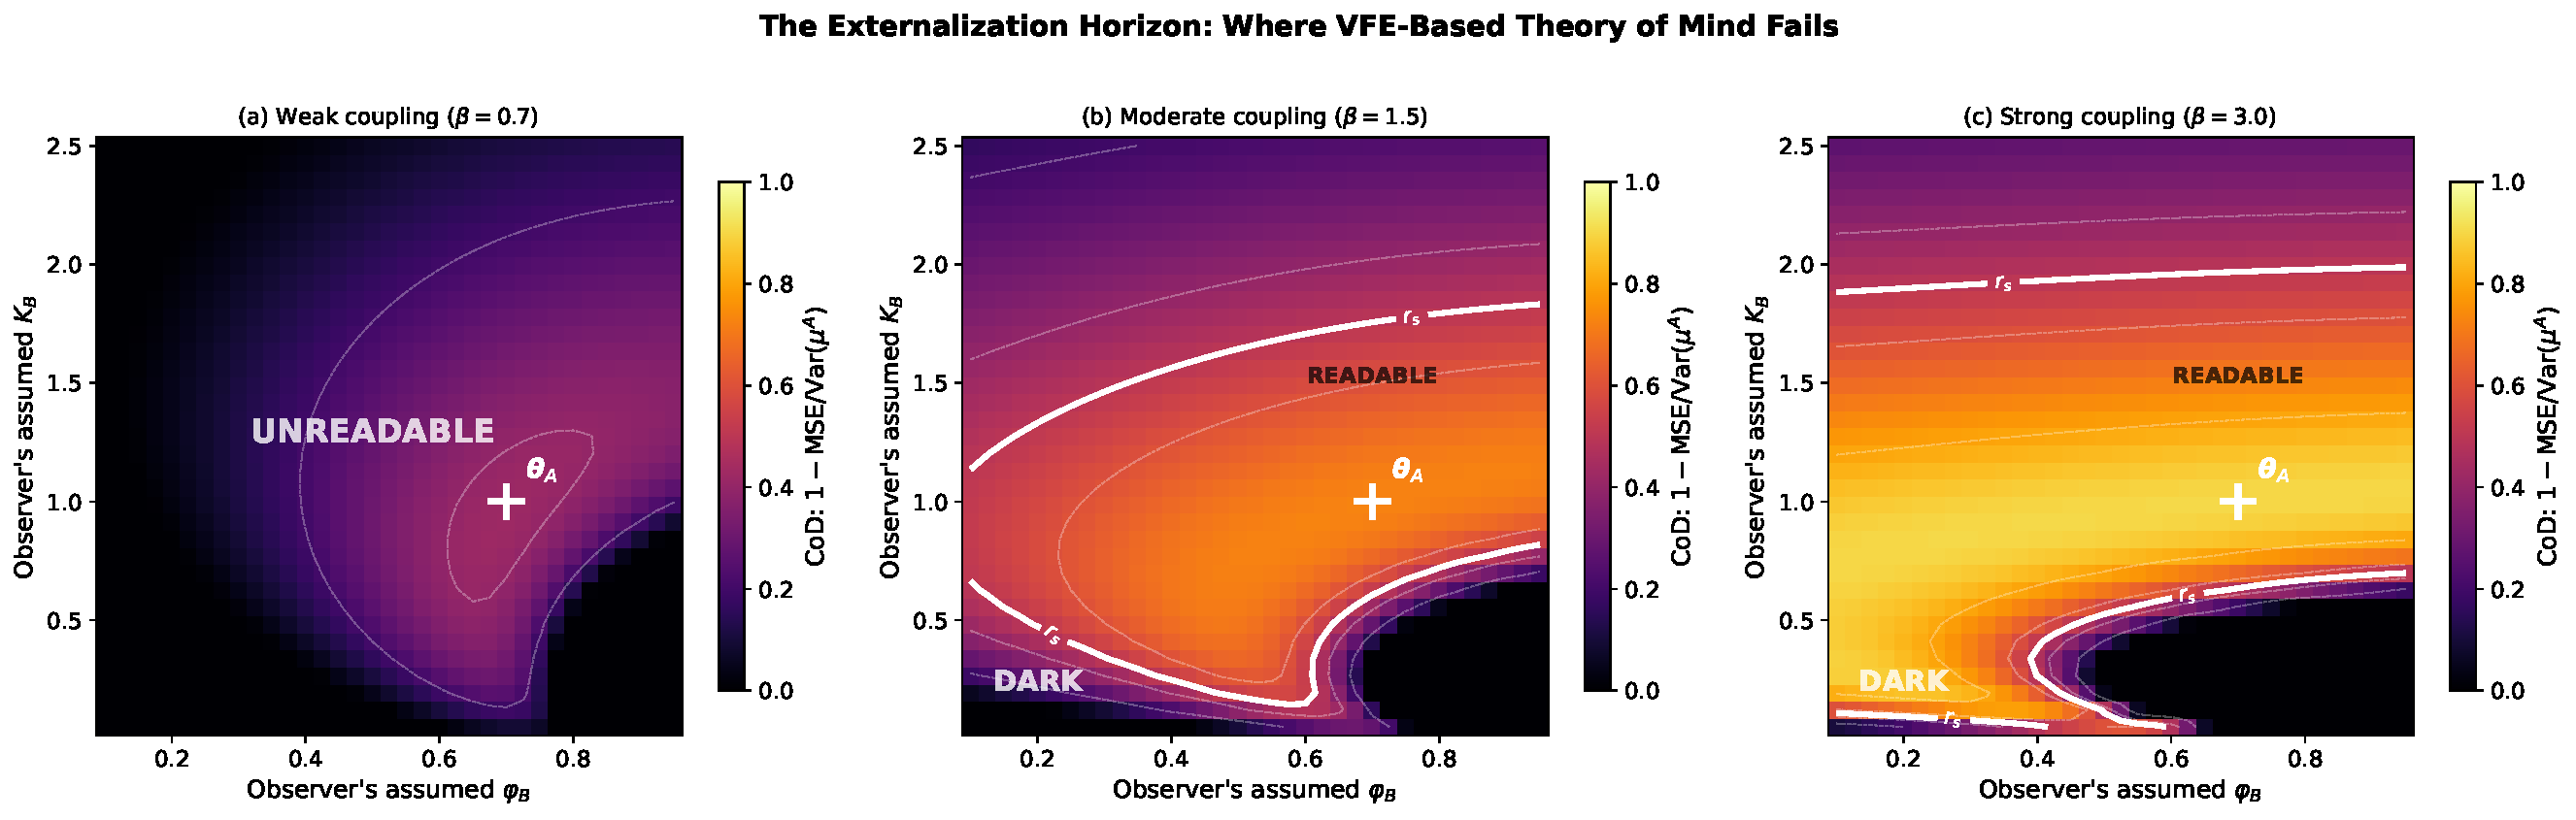
\includegraphics[width=\textwidth]{figures/fig2_horizon_heatmap.pdf}
    \caption{The externalization horizon in model space. Heatmap: $\mathrm{CoD}(\varphi_B, K_B) = 1 - \mathrm{MSE}/\mathrm{Var}(\mu^A)$, where observer $B$ minimizes VFE over a generative model of $A$'s belief dynamics. Unlike $R^2 = \mathrm{corr}^2$, the CoD penalizes scale and bias errors from gain mismatch ($K_B \neq K_A$). White contour: $\mathrm{CoD} = r_s$ (the horizon). White ``+'': matched model $\boldsymbol{\theta}_A$. (a)~Moderate coupling ($\beta = 1.5$): large dark region where ToM fails. (b)~Strong coupling ($\beta = 3.0$): horizon shrinks as externalization increases.}
    \label{fig:horizon}
\end{figure}

\subsection{Observer-Dependent Theory of Mind}

Figure~\ref{fig:observer_dep} validates the key conceptual claim: the same agent can be transparent to one observer and dark to another. Agent~$A$ has fixed parameters $(\varphi = 0.7, K = 1.0)$. Observer~$B_1$ is well-calibrated ($\varphi_{B_1} = 0.7$, $K_{B_1} = 1.0$); observer~$B_2$ is strongly miscalibrated ($\varphi_{B_2} = 0.95$, $K_{B_2} = 0.1$)---expecting a slow, weakly-coupled agent. Both perform VFE minimization over their respective generative models of $A$. Panel~(a): a 200-step time series showing $\mu^A$ (black), $m^{B_1}$ (teal, tracks closely), and $m^{B_2}$ (coral, fails to track). Panel~(b): $R^2$ vs coupling strength $\beta$ for both observers. $B_1$ crosses the readability threshold at lower coupling than $B_2$---the gap between the two curves is the \emph{observer-dependent component} of the horizon, determined entirely by model similarity. Panel~(c): the mechanism underlying the difference. $B_1$'s posterior uncertainty $P_B$ drops well below its prior $P_{\text{prior}}$---observations are informative, VFE minimization succeeds in reducing uncertainty. $B_2$'s posterior remains near the prior---observations are uninformative under the wrong model, and VFE minimization yields no epistemic gain. This is the active inference explanation for why model mismatch produces opacity: when the generative model is wrong, the agent's VFE-optimal inference converges to a systematically biased estimate.

\begin{figure}[htbp]
    \centering
    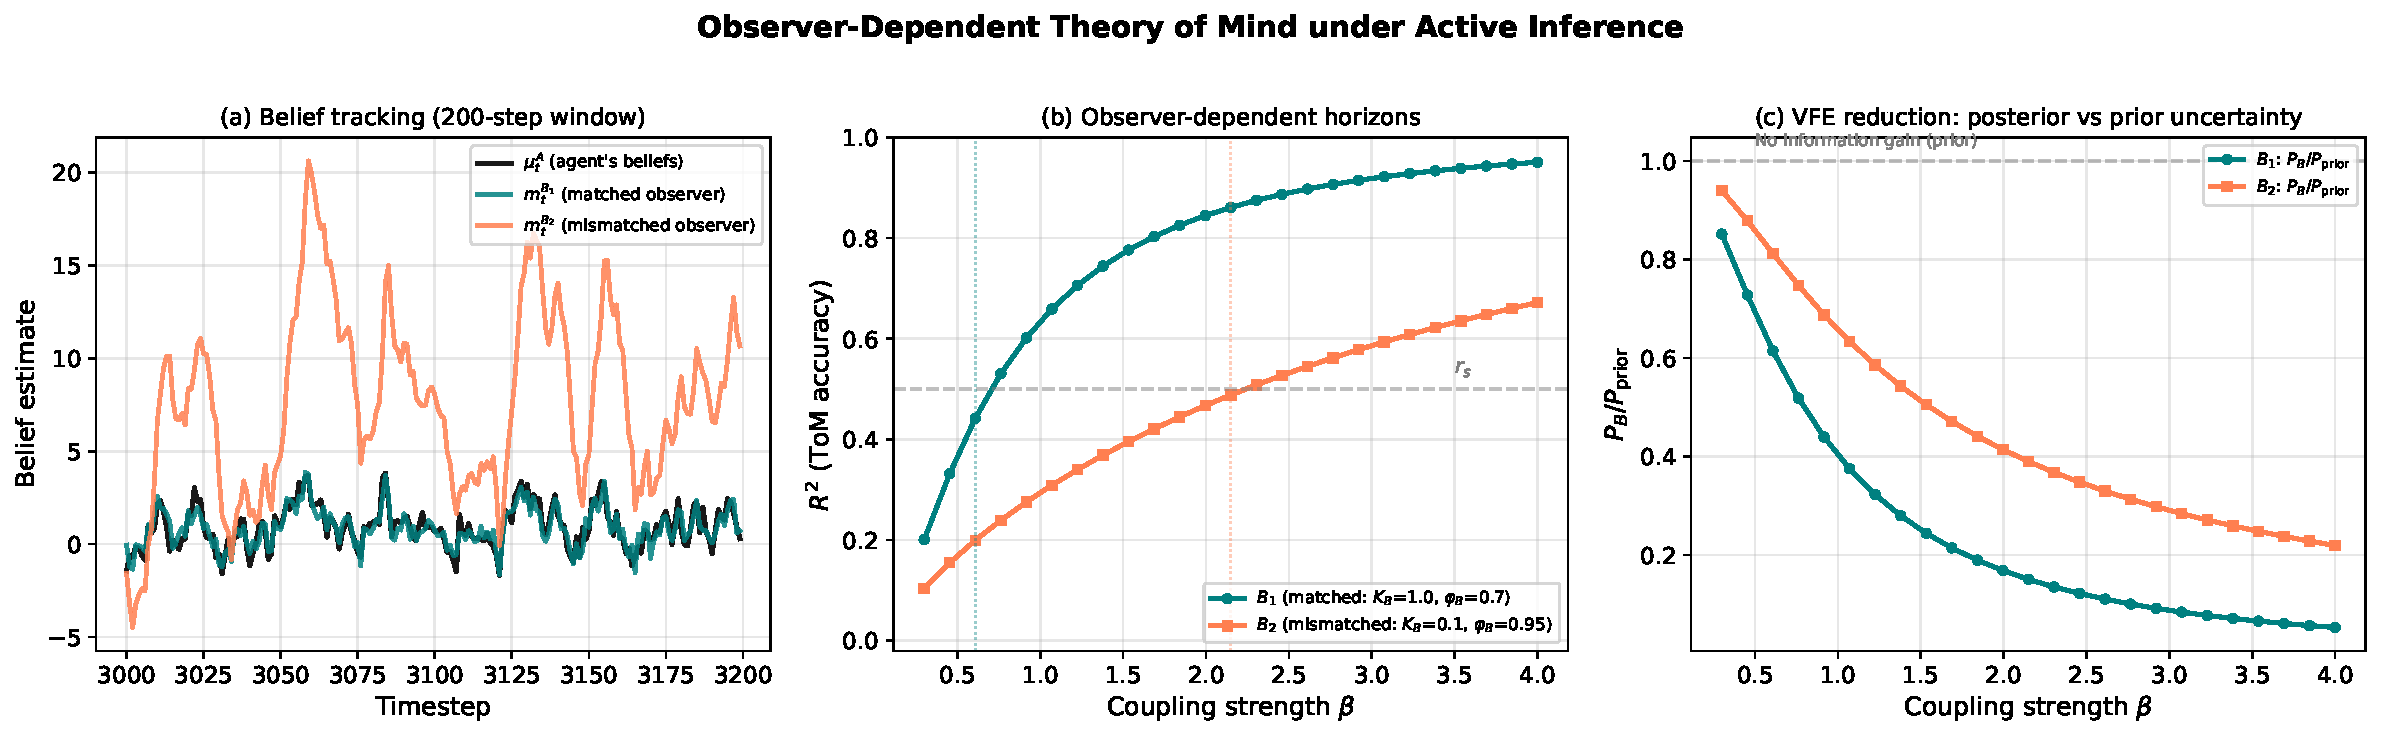
\includegraphics[width=\textwidth]{figures/fig3_observer_dependent.pdf}
    \caption{Observer-dependent Theory of Mind under active inference. (a)~$B_1$ (teal, matched) tracks $\mu^A$ (black); $B_2$ (coral, $K_B\!=\!0.1$, $\varphi_B\!=\!0.95$) does not. (b)~$R^2$ vs coupling $\beta$: $B_1$ crosses threshold at lower coupling. (c)~$P_B/P_{\text{prior}}$: $B_1$'s VFE minimization reduces uncertainty; $B_2$'s does not (posterior $\approx$ prior). Parameters: $\beta = 2.0$, $\sigma_B = 0.5$.}
    \label{fig:observer_dep}
\end{figure}

\subsection{Dynamic Opacity}

Figure~\ref{fig:dynamic} shows what happens when agent~$A$ changes its internal parameters during deployment---a scenario relevant to AGI systems that update their policies online. Agent~$A$'s policy gain $K$ transitions from $1.0$ to $0.3$ and persistence $\varphi$ from $0.7$ to $0.4$ via a sigmoid schedule at $t = T/2$. Observer~$B$ starts with a matched generative model ($\varphi_B = 0.7$, $K_B = 1.0$) and performs VFE minimization throughout, but does not update its model parameters. Panel~(a): $A$'s time-varying parameters (solid) vs $B$'s fixed assumptions (dashed). Panel~(b): Sliding-window $R^2$ drops from the readable regime to the dark regime, crossing the horizon after the parameter change. Panel~(c): The gap between actual MSE and $B$'s reported posterior variance $P^B$ reveals the most concerning consequence: $B$'s VFE-based inference produces \emph{confident but wrong} estimates. The posterior $P^B$ does not increase to reflect the model's degradation, because the Kalman filter's uncertainty estimate is calibrated to the (now incorrect) generative model, not to the actual prediction error. This demonstrates that an observer performing exact VFE minimization under a stale model can be systematically deceived---not by the agent's intention, but by the structural mismatch between model and reality.

\begin{figure}[htbp]
    \centering
    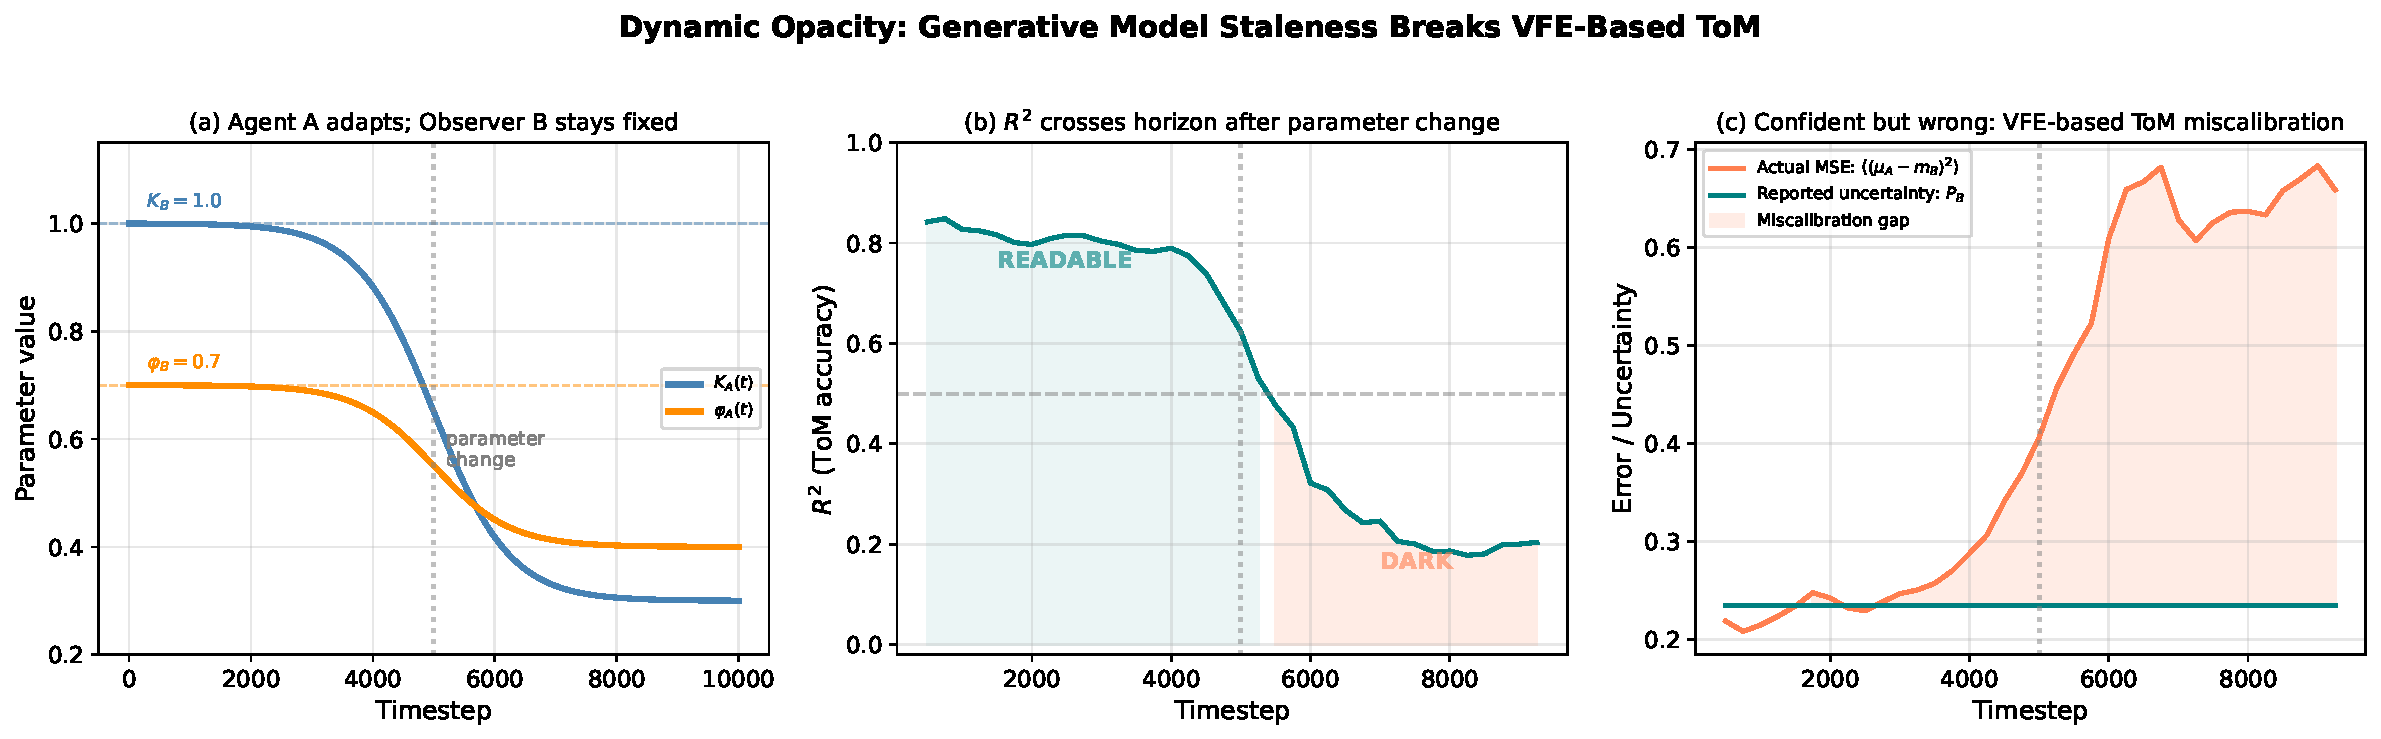
\includegraphics[width=\textwidth]{figures/fig4_dynamic_opacity.pdf}
    \caption{Dynamic opacity: generative model staleness breaks VFE-based ToM. (a)~Agent $A$ changes $K$ and $\varphi$ at $t = T/2$; observer $B$ stays fixed. (b)~$R^2$ crosses the horizon: readable $\to$ dark. (c)~Actual MSE (coral) diverges from reported $P_B$ (teal)---$B$'s VFE minimization produces confident but wrong estimates (shaded gap).}
    \label{fig:dynamic}
\end{figure}

%% ============================================================
\section{Discussion}
\label{sec:discussion}
%% ============================================================

\subsection{Interpretability as a Relation}

The externalization horizon reframes AGI interpretability as fundamentally \emph{relational}. Current approaches focus on properties of the system: architectural transparency (attention visualization), post-hoc explanation (SHAP values), or mechanistic interpretability (circuit analysis). Our framework asks a different question: interpretable \emph{to whom}? An AGI system operating below the externalization horizon is dark not because we lack tools, but because the observer's model of the system is insufficiently accurate. This has direct implications for AI safety: alignment verification requires not only that the agent externalize its goals, but that the auditor have an adequate model of \emph{how} the agent maps beliefs to actions. A well-calibrated auditor (small $|\boldsymbol{\delta}|$) can verify alignment at lower coupling strength than a poorly calibrated one.

\subsection{Innovation Consistency as a Diagnostic}

Our results reveal that standard metrics like squared correlation ($R^2 = \mathrm{corr}^2$) can be misleading for assessing model quality. Because $R^2$ is scale-invariant, an observer with a severely mismatched gain $K_B$ can produce estimates that correlate with $\mu^A$ (since the Kalman filter's observation update partially compensates) yet are systematically biased and mis-scaled---yielding high $R^2$ but near-zero or negative CoD. This motivates our use of the coefficient of determination ($\mathrm{CoD} = 1 - \mathrm{MSE}/\mathrm{Var}$) for the horizon heatmaps (Figure~\ref{fig:horizon}). More broadly, the Kalman filter's observation update can mask transition model errors, maintaining reasonable correlation even when the observer's generative model is structurally wrong. The innovation consistency ratio ($\mathrm{ICR} = \mathrm{Var}(\text{innov})/S$) provides a complementary diagnostic that detects misspecification invisible to correlation. Figure~\ref{fig:dynamic}(c) illustrates a related pathology: the observer's posterior uncertainty $P^B$ remains flat even as actual prediction error spikes, because the uncertainty estimate is calibrated to the (incorrect) model rather than to reality. This suggests a practical protocol for AGI monitoring: track not only whether your model of the system correlates with its behavior, but whether your model's \emph{predictions} are calibrated---innovations should be white noise with variance matching the predicted innovation variance.

\subsection{Connection to Empowerment and Agency}

Our controllability measure $\mathcal{R}_a$ is closely related to empowerment \cite{klyubin2005empowerment} but with a crucial distinction. Empowerment maximizes $I(a_t; s_{t+1})$---the channel capacity from actions to states. Our measure computes $I(\mu_t; e_{t+1})$---the actual information flow from beliefs to environment under the current policy. This parallels the distinction between Kolchinsky and Wolpert's~\cite{kolchinsky2018semantic} viability \emph{value} of information (the minimum required for self-maintenance) and the actual information rate. An agent is genuinely ``agentic'' not merely when it \emph{could} influence the world (empowerment), but when it \emph{does} influence the world through its beliefs (externalization).

\subsection{The Robot as Stranger}

Our framework formalizes a concern raised in recent discussions of synthetic neurophenomenology \cite{monnier2025generative}: the robot is fundamentally a ``stranger.'' In the model-similarity framework, this opacity has a precise source: the human's generative model of the robot's dynamics---$(\varphi_B, v_B, K_B)$---is likely far from the robot's actual parameters. The robot may heavily externalize ($\mathcal{E}$ well above threshold), yet remain unreadable because the human's model of \emph{how} the robot maps beliefs to actions is wrong. The mutual readability $\mathcal{M}(A, B)$ (eq.~\ref{eq:mutual_readability}) quantifies this: even if both agents externalize strongly, mutual comprehension requires that each has an adequate model of the other. Figure~\ref{fig:observer_dep} illustrates this directly: the same agent is transparent to $B_1$ and dark to $B_2$.

\subsection{Dynamic Opacity and Model Staleness}

Figure~\ref{fig:dynamic} demonstrates a scenario particularly relevant to deployed AGI: an agent that changes its internal parameters---through online learning, policy updates, or environmental adaptation---becomes progressively opaque to an observer calibrated on pre-change behavior. The miscalibration gap (actual MSE vs reported $P^B$) is especially concerning: the observer's \emph{confidence} in its model of the agent does not degrade, even as the model's accuracy collapses. This suggests that monitoring systems for AGI should track not only model fit but model \emph{freshness}---the time since the observer's model was last validated against the agent's actual dynamics.

\subsection{Connection to Phenomenological Privacy}

If some internal states are \emph{in principle} beyond the externalization horizon, the horizon provides a formal boundary between the \textbf{communicable} (states above the horizon, accessible through externalization and inference) and the \textbf{private} (states below the horizon, causally disconnected from the observable world). This is not a claim about consciousness per se, but a structural observation: the externalization horizon partitions cognitive states into those that can participate in shared reality and those that cannot. Whether the ``private'' states constitute subjective experience is a question our framework poses but does not answer.

\subsection{Limitations and Future Work}

Our analysis is limited to linear-Gaussian systems where closed-form results are available. Key extensions include: (i)~\textbf{nonlinear systems} with state-dependent horizons, where the 2026 differential flatness framework for active inference \cite{friston2026flatness} may provide analytical handles; (ii)~\textbf{hierarchical models} where different levels of a deep temporal model may have different externalization radii; (iii)~\textbf{active deception}---an agent that deliberately selects dynamics to maximize $|\boldsymbol{\delta}|$ for specific observers, formalizing strategic opacity; (iv)~\textbf{empirical validation} in embodied robotic systems; and (v)~\textbf{model learning}---extending the framework to observers that update $\boldsymbol{\theta}_B$ online, creating an arms race between agent adaptation and observer calibration.

%% ============================================================
\section{Conclusion}
\label{sec:conclusion}
%% ============================================================

We have introduced the externalization horizon: an information-theoretic boundary that determines when an active inference agent's internal states can be inferred by an external observer. Our key insight is that this boundary is \textbf{observer-dependent}: readability emerges from the similarity between the observer's generative model and the agent's actual dynamics, not from a property of the agent alone. We showed that (i)~policy gain mismatch dominates readability degradation through the observation model; (ii)~innovation consistency detects model misspecification invisible to correlation; and (iii)~dynamic parameter changes, feedback coupling, and observer calibration all reshape the horizon in parameter space.

The externalization horizon provides a unified language for questions spanning AGI interpretability (when can we read an AI's goals---and \emph{who} can read them?), multi-agent coordination (when can agents model each other?), and the philosophy of mind (what is the boundary between communicable and private cognitive states?). By moving beyond the binary question of ``does a boundary exist?'' to the relational question of ``who can see through the boundary, and how does that depend on their model of the agent?,'' we open new avenues for understanding the conditions under which minds---biological or artificial---become mutually intelligible.

%% ============================================================
% Bibliography
%% ============================================================

\bibliographystyle{splncs04}
\begin{thebibliography}{99}

\bibitem{friston2006free}
Friston, K., Kilner, J., Harrison, L.: A free energy principle for the brain. J. Physiol.\ Paris \textbf{100}(1--3), 70--87 (2006)

\bibitem{friston2010free}
Friston, K.: The free-energy principle: a unified brain theory? Nat. Rev. Neurosci. \textbf{11}(2), 127--138 (2010)

\bibitem{parr2022active}
Parr, T., Pezzulo, G., Friston, K.J.: Active Inference: The Free Energy Principle in Mind, Brain, and Behavior. MIT Press (2022)

\bibitem{parr2019generalized}
Parr, T., Friston, K.: Generalised free energy and active inference. Biol. Cybern. \textbf{113}, 495--513 (2019)

\bibitem{pearl1988probabilistic}
Pearl, J.: Probabilistic Reasoning in Intelligent Systems. Morgan Kaufmann (1988)

\bibitem{friston2013life}
Friston, K.: Life as we know it. J. R. Soc. Interface \textbf{10}(86), 20130475 (2013)

\bibitem{kirchhoff2018markov}
Kirchhoff, M., Parr, T., Palacios, E., Friston, K., Kiverstein, J.: The Markov blankets of life: autonomy, active inference and the free energy principle. J. R. Soc. Interface \textbf{15}(138), 20170792 (2018)

\bibitem{ramstead2023bayesian}
Ramstead, M.J.D., Sakthivadivel, D.A.R., Heins, C., et al.: On Bayesian mechanics: a physics of and by beliefs. Interface Focus \textbf{13}(3), 20220029 (2023)

\bibitem{bruineberg2022emperor}
Bruineberg, J., Dolega, K., Dewhurst, J., Baltieri, M.: The Emperor's New Markov Blankets. Behav. Brain Sci. \textbf{45}, e183 (2022)

\bibitem{raja2021free}
Raja, V., Valluri, D., Baggs, E., Chemero, A., Anderson, M.L.: The Markov blanket trick: on the scope of the free energy principle and active inference. Phys. Life Rev. \textbf{39}, 49--72 (2021)

\bibitem{biehl2021technical}
Biehl, M., Pollock, F.A., Kanai, R.: A technical critique of some parts of the free energy principle. Entropy \textbf{23}(3), 293 (2021)

\bibitem{aguilera2022particular}
Aguilera, M., Millidge, B., Tschantz, A., Buckley, C.L.: How particular is the physics of the free energy principle? Phys. Life Rev. \textbf{40}, 24--50 (2022)

\bibitem{aguilera2023knitting}
Aguilera, M., Millidge, B., Tschantz, A., Buckley, C.L.: Knitting a Markov blanket is hard when you are out-of-equilibrium. In: Active Inference, pp.~59--73. Springer (2023)

\bibitem{parr2020information}
Parr, T., Da Costa, L., Friston, K.: Markov blankets, information geometry and stochastic thermodynamics. Phil. Trans. R. Soc. A \textbf{378}(2164), 20190159 (2020)

\bibitem{possati2025density}
Possati, L.M.: Markov blanket density and free energy minimization. arXiv:2506.05794 (2025)

\bibitem{sakthivadivel2022weak}
Sakthivadivel, D.A.R.: Weak Markov blankets in high-dimensional, sparsely-coupled random dynamical systems. arXiv:2207.07620 (2022)

\bibitem{klyubin2005empowerment}
Klyubin, A.S., Polani, D., Nehaniv, C.L.: Empowerment: a universal agent-centric measure of control. In: IEEE Congress on Evolutionary Computation, pp.~128--135 (2005)

\bibitem{salge2014empowerment}
Salge, C., Glackin, C., Polani, D.: Empowerment---an introduction. In: Guided Self-Organization: Inception, pp.~67--114. Springer (2014)

\bibitem{kiefer2025empowerment}
Kiefer, A.: Empowerment, free energy, and causal path entropy are the same thing. Entropy \textbf{27}(4) (2025)

\bibitem{schreiber2000measuring}
Schreiber, T.: Measuring information transfer. Phys. Rev. Lett. \textbf{85}(2), 461 (2000)

\bibitem{barnett2009granger}
Barnett, L., Barrett, A.B., Seth, A.K.: Granger causality and transfer entropy are equivalent for Gaussian variables. Phys. Rev. Lett. \textbf{103}(23), 238701 (2009)

\bibitem{ay2008information}
Ay, N., Polani, D.: Information flows in causal networks. Adv. Complex Syst. \textbf{11}(1), 17--41 (2008)

\bibitem{kolchinsky2018semantic}
Kolchinsky, A., Wolpert, D.H.: Semantic information, autonomous agency and non-equilibrium statistical physics. Interface Focus \textbf{8}(6), 20180041 (2018)

\bibitem{lizier2008phase}
Lizier, J.T., Prokopenko, M., Zomaya, A.Y.: Local information transfer as a spatiotemporal filter for complex systems. Phys. Rev. E \textbf{77}(2), 026110 (2008)

\bibitem{baker2017rational}
Baker, C.L., Jara-Ettinger, J., Saxe, R., Tenenbaum, J.B.: Rational quantitative attribution of beliefs, desires and percepts in human mentalizing. Nat. Hum. Behav. \textbf{1}(4), 0064 (2017)

\bibitem{rabinowitz2018machine}
Rabinowitz, N., Perbet, F., Song, H.F., Zhang, C., Eslami, S.M.A., Botvinick, M.: Machine theory of mind. In: ICML, PMLR \textbf{80}, pp.~4218--4227 (2018)

\bibitem{friston2015duet}
Friston, K., Frith, C.: A duet for one. Conscious. Cogn. \textbf{36}, 390--405 (2015)

\bibitem{veissiere2020thinking}
Veissi\`{e}re, S.P.L., Constant, A., Ramstead, M.J.D., Friston, K.J., Kirmayer, L.J.: Thinking through other minds: a variational approach to cognition and culture. Behav. Brain Sci. \textbf{43}, e90 (2020)

\bibitem{vasil2020communication}
Vasil, J., Badcock, P.B., Constant, A., Friston, K., Ramstead, M.J.D.: A world unto itself: human communication as active inference. Front. Psychol. \textbf{11}, 417 (2020)

\bibitem{maisto2023interactive}
Maisto, D., Donnarumma, F., Pezzulo, G.: Interactive inference: a multi-agent model of cooperative joint actions. IEEE Trans. Syst. Man Cybern.: Systems (2023)

\bibitem{albarracin2024protentions}
Albarracin, M., Pitliya, R.J., St~Clere~Smithe, T., Friedman, D.A., Friston, K., Ramstead, M.J.D.: Shared protentions in multi-agent active inference. Entropy \textbf{26}(4), 303 (2024)

\bibitem{albarracin2026empathy}
Albarracin, M., Mikeda, A., Jimenez~Rodriguez, A., et al.: Empathy modeling in active inference agents for perspective-taking and alignment. arXiv:2602.20936 (2026)

\bibitem{monnier2025generative}
Monnier, A., Adel, L., Dumas, G.: Now is the time: operationalizing generative neurophenomenology through interpersonal methods. Neurosci. Conscious. \textbf{2025}(1), niaf052 (2025)

\bibitem{varela1996neurophenomenology}
Varela, F.J.: Neurophenomenology: a methodological remedy for the hard problem. J. Conscious. Stud. \textbf{3}(4), 330--349 (1996)

\bibitem{ramstead2022generative}
Ramstead, M.J.D., Seth, A.K., Hesp, C., et al.: From generative models to generative passages: a computational approach to (neuro) phenomenology. Rev. Philos. Psychol. \textbf{13}(4), 829--857 (2022)

\bibitem{sandvedsmith2025deep}
Sandved-Smith, L., Bogota, J.D., Hohwy, J., Kiverstein, J., Lutz, A.: Deep computational neurophenomenology: a methodological framework. Neurosci. Conscious. \textbf{2025}(1), niaf016 (2025)

\bibitem{friston2008variational}
Friston, K.: Variational filtering. NeuroImage \textbf{41}(3), 747--766 (2008)

\bibitem{baltieri2020kalman}
Baltieri, M., Buckley, C.L.: On Kalman-Bucy filters, linear quadratic control and active inference. arXiv:2005.06269 (2020)

\bibitem{koudahl2021efe}
Koudahl, M.T., Kouw, W.M., de~Vries, B.: On epistemics in expected free energy for linear Gaussian state space models. Entropy \textbf{23}(12), 1565 (2021)

\bibitem{cover2006elements}
Cover, T.M., Thomas, J.A.: Elements of Information Theory, 2nd edn. Wiley (2006)

\bibitem{baltieri2020bayesian}
Baltieri, M., Buckley, C.L.: A Bayesian perspective on classical control. arXiv:2004.10288 (2020)

\bibitem{dragan2013legibility}
Dragan, A.D., Lee, K.C.T., Srinivasa, S.S.: Legibility and predictability of robot motion. In: HRI '13, pp.~301--308. ACM/IEEE (2013)

\bibitem{friston2026flatness}
Friston, K., Mounier, H., et al.: Active inference and functional parametrisation: differential flatness and smooth random realisation. Entropy \textbf{28}(1), 87 (2026)

\bibitem{dacosta2020discrete}
Da~Costa, L., Parr, T., Sajid, N., Veseli\'{c}, S., Neacsu, V., Friston, K.: Active inference on discrete state-spaces: a synthesis. J. Math. Psychol. \textbf{99}, 102447 (2020)

\bibitem{friston2012optimal}
Friston, K., Samothrakis, S., Montague, R.: Active inference and agency: optimal control without cost functions. Biol. Cybern. \textbf{106}, 523--541 (2012)

\bibitem{dacosta2021neural}
Da~Costa, L., Parr, T., Sengupta, B., Friston, K.: Neural dynamics under active inference: plausibility and efficiency of information processing. Entropy \textbf{23}(4), 454 (2021)

\end{thebibliography}

\end{document}
